% f-transformer-flow — pure-Transformer EPF model, after Llorente & Portela (2025), Fig. 2a.
% Standalone TikZ figure: compile with pdflatex/lualatex. Caption lives in the chapter.
\documentclass[tikz,border=6pt]{standalone}
\usetikzlibrary{positioning, arrows.meta, calc}

\begin{document}
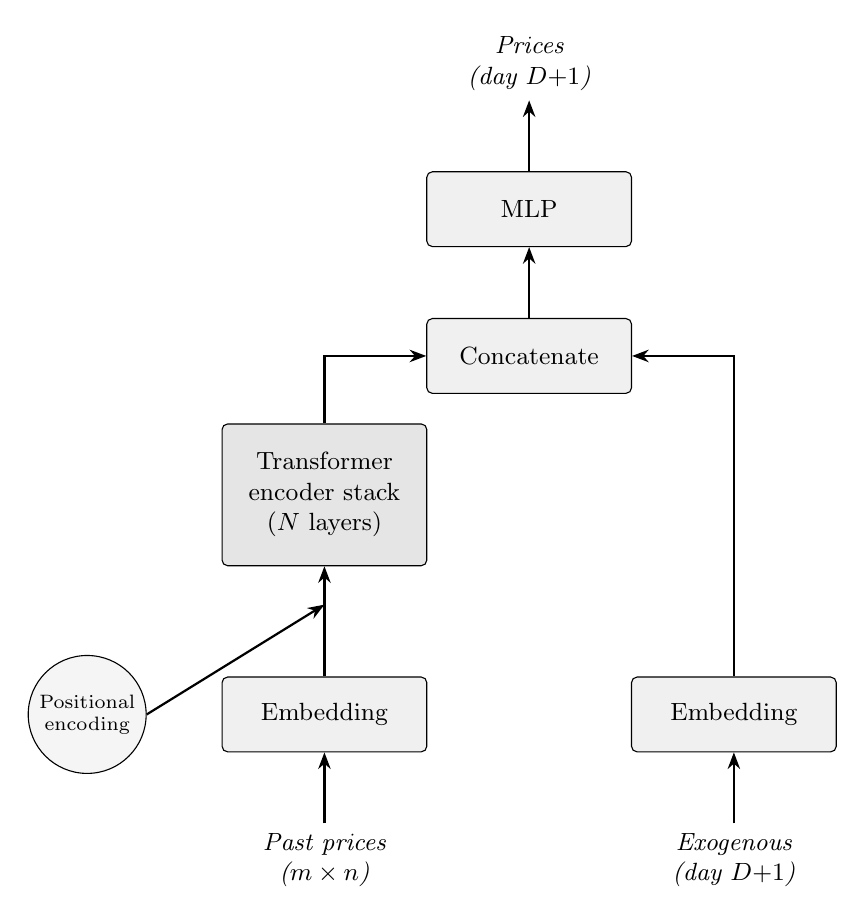
\begin{tikzpicture}[
  >={Stealth[length=6pt]},
  blk/.style={draw, rectangle, rounded corners=2pt, minimum width=2.6cm,
              minimum height=0.95cm, align=center, font=\small, fill=gray!12},
  tall/.style={blk, minimum height=1.8cm, fill=gray!20},
  io/.style={align=center, font=\small\itshape},
  pe/.style={draw, circle, align=center, font=\scriptsize, fill=gray!8, inner sep=2pt},
  arr/.style={->, thick},
]

% ---- price branch (left) ----
\node[io]   (pin)  at (0,0)             {Past prices\\($m\times n$)};
\node[blk]  (pemb) [above=0.9cm of pin] {Embedding};
\node[tall] (enc)  [above=1.4cm of pemb]{Transformer\\encoder stack\\($N$ layers)};

% positional encoding merging into the price path
\node[pe] (pe) [left=0.95cm of pemb] {Positional\\encoding};

% ---- exogenous branch (right) ----
\node[io]  (xin)  at (5.2,0)           {Exogenous\\(day $D{+}1$)};
\node[blk] (xemb) [above=0.9cm of xin] {Embedding};

% ---- merge + head ----
\node[blk] (cat) at (2.6,6.4)        {Concatenate};
\node[blk] (mlp) [above=0.9cm of cat]{MLP};
\node[io]  (out) [above=0.9cm of mlp]{Prices\\(day $D{+}1$)};

% ---- arrows ----
\draw[arr] (pin)  -- (pemb);
\draw[arr] (pemb) -- (enc);
\draw[arr] (pe.east) -- ($(pemb)!0.5!(enc)$);   % positional encoding into the price path
\draw[arr] (xin)  -- (xemb);
\draw[arr] (enc.north)  |- (cat.west);
\draw[arr] (xemb.north) |- (cat.east);
\draw[arr] (cat) -- (mlp);
\draw[arr] (mlp) -- (out);

\end{tikzpicture}
\end{document}
